\documentclass[12pt,a4paper]{article}
%<--------------------------------------------------------------------------->%
%%% CJK %%%
\usepackage{xeCJK}
\setCJKmainfont{GenWanMin TJ L}
\setCJKsansfont{Noto Sans CJK KR Medium}
%<--------------------------------------------------------------------------->%
%%% TikZ %%%
\usepackage{tikz}
\usetikzlibrary{calc}
\usetikzlibrary{angles,quotes}
\usetikzlibrary{intersections,topaths}
\usetikzlibrary{decorations.markings}
%<--------------------------------------------------------------------------->%
\def\MarkRightAngle[size=#1,dirac=#2](#3,#4,#5){\draw($(#4)!#1cm!(#5)$)--%
($($(#4)!#1cm!(#5)$)!#1cm!#2*(-90):(#5)$)--($(#4)!#1cm!(#3)$);}
%<--------------------------------------------------------------------------->%
%%% blob %%%
\newcommand{\blob}[2]{%
	\draw[fill opacity=.4,fill=red,draw=none,rounded corners=#1*1mm]%
	(#2) +($(0:#1*2+#1*rnd)$)%
	\foreach \a in {20,40,...,350} { -- +($(\a: #1*2+#1*rnd)$) } -- cycle;%
}
%<--------------------------------------------------------------------------->%
%%% get coordinate %%%
\draw let \p{B}=(B) in coordinate (C) at (\x{B},-\y{B});
%<--------------------------------------------------------------------------->%
%%% detailed label positioning %%%
\node[bai,label={[shift={(0.1,0)}]{$a$}}] at (a) {};
%<--------------------------------------------------------------------------->%

\begin{document}

% \begin{tikzpicture}
% 	\draw (0,0) circle [radius=0.5];
% 	\draw[->,thick] (0,0)--(45:0.5) {r};
% \end{tikzpicture}

\begin{tikzpicture}[scale=3] %% tikz nodes
	\tikzstyle{transition}=[circle,draw=blue!50,fill=blue!20,thick,inner sep=2pt,minimum size=6mm];
	\tikzstyle{place}=[rectangle,draw=black!50,fill=black!20,thick,inner sep=2pt,minimum size=4mm];
	\node[transition] (B) at (0,0) {B};
	\node[transition] (A) at (0,.5) {我};
	\node[transition] (C) [below of=B] {C};
	\node[place]      (D) [right of=B] {D}
		edge [->,bend right=45] node[auto,swap]{$r$} (A)
		edge [<-,bend left=45] (C)
		edge [<-] (B);
	\node[place]      (E) [left of=B]  {E}
		edge [<-,bend left=45]
			node[auto,swap]{$r$}
			node[auto]{$s$}
			(A)
		edge  [->,bend right=45](C)
		edge [->] (B);
\end{tikzpicture}

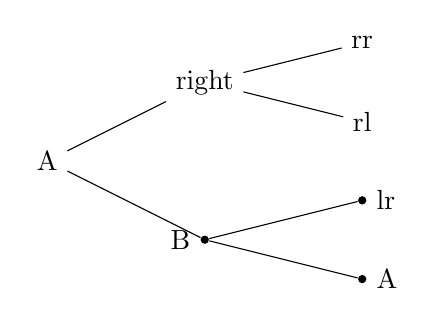
\begin{tikzpicture}[grow=right] %% tikz tree
	% \tikzset{
	% solid node/.style={circle,draw,inner sep=1.2,fill=black},
	% hollow node/.style={circle,draw,inner sep=1.2},
	% }
	\tikzstyle{level 1}=[level distance=2cm, sibling distance=2cm];
	\tikzstyle{level 2}=[level distance=2cm, sibling distance=1cm];
	\tikzstyle{temp}=[circle,inner sep=0pt,minimum width=3pt,fill]
	\node {A}
		child {
			node[temp,label=left:B]{}
			child { node[temp,label=right:A] {} }
			child { node[temp,label=right:lr]{} }
		}
		child {
			node {right}
			child { node {rl} }
			child { node {rr} }
		};
\end{tikzpicture}

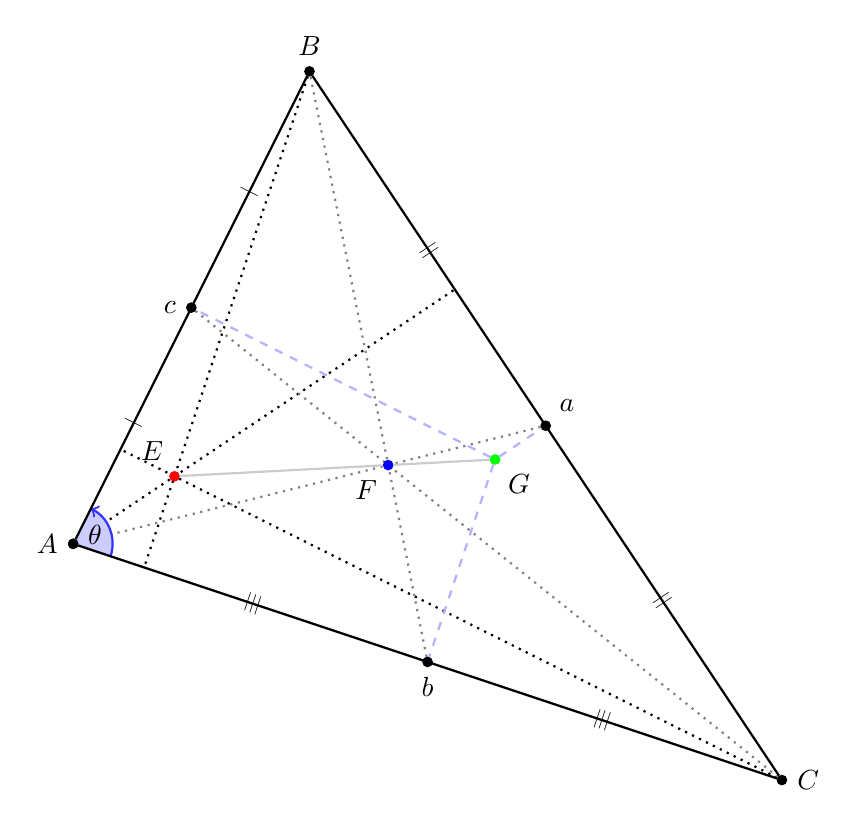
\begin{tikzpicture}[thick,scale=3] %% tikz
	\tikzstyle{jiao}=[draw,circle,fill,inner sep=0pt,minimum width=3pt];
	%% points
	\node[label=left:$A$,jiao] (AA) at (0,0) {};
	\node[label=above:$B$,jiao] (BB) at (1,2) {};
	\node[label=right:$C$,jiao] (CC) at (3,-1){};
	%% how to put label "mid arc": use `midway` option.
	%% projection
	\draw[dotted] (AA) -- ($(BB)!(AA)!(CC)$) coordinate (aa);
	\draw[dotted] (BB) -- ($(AA)!(BB)!(CC)$) coordinate (bb);
	\draw[dotted] (CC) -- ($(BB)!(CC)!(AA)$) coordinate (cc);
	%% coordinate calculation
	\node[jiao,label=left:$c$] (AB) at ($(AA)!0.5!(BB)$) {};
	\node[jiao,label=above right:$a$] (BC) at ($(BB)!0.5!(CC)$) {};
	\node[jiao,label=below:$b$] (AC) at ($(AA)!0.5!(CC)$) {};
	\draw[dotted,black!50] (AB) -- (CC);
	\draw[dotted,black!50] (BC) -- (AA);
	\draw[dotted,black!50] (AC) -- (BB);
	\coordinate (Bb) at ($(AC)!1cm!90:(CC)$);
	\coordinate (Aa) at ($(BC)!1cm!90:(BB)$);
	%% centers
	\node[blue] (F) [jiao,label=260:$F$] at (intersection of AB--CC and BC--AA) {};
	\node[red] (E) [jiao,label=100:$E$] at (intersection of BB--bb and AA--aa) {};
	\node[green] (G) [jiao,label=-60:$G$] at (intersection of AC--Bb and BC--Aa) {};
	%% perpendicular bisectors
	\draw[blue!30,dashed] (G)--(AC);
	\draw[blue!30,dashed] (G)--(BC);
	\draw[blue!30,dashed] (G)--(AB);
	%% highway
	\draw[black!20] (F) -- (E);
	\draw[black!20] (G) -- (F);
	%% angle
	\pic ["$\theta$",->,draw=blue!80,fill=blue!20] {angle = CC--AA--BB};
	%% mark right angle
	\MarkRightAngle[size=0.06,dirac=1](AA,aa,CC);
	\MarkRightAngle[size=0.06,dirac=-1](BB,bb,CC);
	\MarkRightAngle[size=0.06,dirac=1](CC,cc,BB);
	%% draw triangle
	\draw
		(AA) node[jiao]{} --
			node[pos=1/4,sloped,scale=.7]{$|$}
			node[pos=3/4,sloped,scale=.7]{$|$}
		(BB) --
			node[pos=1/4,sloped,scale=.7]{$||$}
			node[pos=3/4,sloped,scale=.7]{$||$}
		(CC) --
			node[pos=1/4,sloped,scale=.7]{$|||$}
			node[pos=3/4,sloped,scale=.7]{$|||$} (AA) ;
\end{tikzpicture}

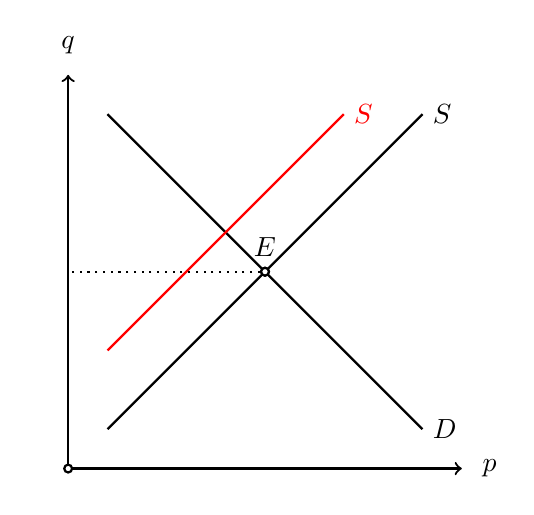
\begin{tikzpicture}[thick,scale=1/2] %% tikz
	\tikzstyle{jiao}=[circle,draw,fill=white,inner sep=1pt];
	\draw[<->] (0,10) node[label=above:$q$]{}  -- (0,0) node[jiao]{} -- (10,0) node[label=right:$p$]{};
	%% curves
	\draw[name path=S] (1,1) -- (9,9) node[anchor=west]{$S$};
	\draw[name path=D] (1,9) -- (9,1) node[anchor=west]{$D$};
	\draw[xshift=-2cm,red] (1,1)++(2,2) -- (9,9) node[anchor=west]{$S$} ;
	\path[name intersections={of=S and D}]; %% name the intersection
	\node[jiao,label=above:$E$] (equi) at (intersection-1) {};
	\draw (equi) edge[dotted] ($(0,0)!(equi)!(0,10)$) node[jiao]{};
\end{tikzpicture}

\begin{figure}[t]
	\centering
	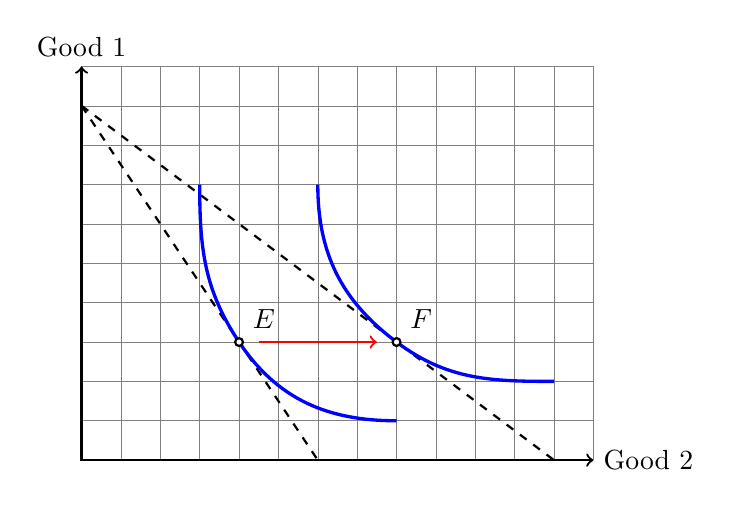
\begin{tikzpicture}[scale=1/2,thick] %% tikz
		\tikzstyle{kong}=[circle,draw,fill=white,inner sep=1pt]
		\tikzstyle{shi}=[circle,draw,fill=white,inner sep=1pt]
		%% axis and grid
		\draw[step=1,help lines] (0,0) grid (13,10);
		\draw[<->] (0,10) node[anchor=south]{Good 1} --(0,0) --(13,0) node[anchor=west]{Good 2};
		% \foreach \x in {1,...,12} {\node[label=below:{\tiny\x},sloped] at (\x,0) {\tiny$|$};}
		% \foreach \x in {1,...,9} {\node[label=above:{\tiny\x},rotate=90] at (0,\x) {\tiny$|$};}
		%% budget curve
		\draw[dashed] (0,9)--(6,0);
		\draw[dashed] (0,9)--(12,0);
		%% first indifference
		\pgfmathsetmacro\tangle{atan2(9,-6)};
		\draw[blue,very thick] (3,7)
			to[in=\tangle,out=-90]     (4,3)
			to[in=180,out=\tangle+180] (8,1);
		%% second indifference
		\pgfmathsetmacro\tangle{atan2(9,-12)};
		\draw[blue,very thick] (6,7)
			to[in=\tangle,out=-90]     (8,3)
			to[in=180,out=\tangle+180] ($(12,1)+(0,1)$);
		%% tangent nodes
		\node[kong,label=above right:$E$] (E) at (4,3) {};
		\node[kong,label=above right:$F$] (F) at (8,3) {};
		%% arrow
		\draw[->,red] (E)++(.5,0) -- ($(F)+(-.5,0)$);
	\end{tikzpicture}
	\caption{Budget constraint shift}
\end{figure}

\begin{tikzpicture}[scale=1/2,decoration={markings,mark=at position 1cm with{\draw (-20pt,0)--(20pt,0);}}] %% tikz
	\draw[postaction={decorate}] (0,0) to[in=10,out=90] (10,9);
\end{tikzpicture}

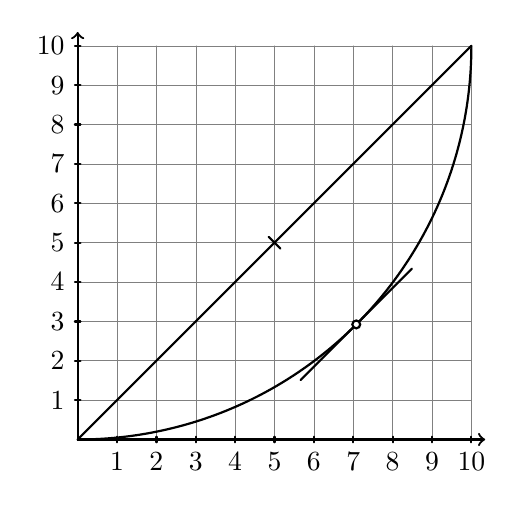
\begin{tikzpicture}[scale=1/2,thick,line cap=round] %% tikz
	\tikzstyle{kong}=[circle,draw,fill=white,inner sep=1pt];
	\tikzstyle{shi}=[circle,fill=black,inner sep=1pt];
	%% axis
	\draw[help lines] (0,0) grid (10,10);
	\foreach \x in {1,...,10} \draw (\x,0) ++(0,2pt) -- +(0,-4pt) node[below]{\x};
	\foreach \x in {1,...,10} \draw (0,\x) ++(2pt,0) -- +(-4pt,0) node[left]{\x};
	% \draw[<->] ($(0,10)+(0,10pt)$) -- (0,0) -- ($(10,0)+(10pt,0)$);
	\draw[<->] (0,10) +(0,10pt) -- (0,0) -- +(10cm+10pt,0);
	% \draw[domain=0:10,smooth] plot (\x,{1/10 * \x * \x}) node[pos=.8,kong]{};
	\draw (0,0) edge[out=0,in=-90] pic[pos=0.5,sloped]{code={\draw (-1,0)-- node[pos=.5,kong]{} (1,0);}} (10,10);
	\draw (0,0) edge pic[pos=0.5,sloped]{code={\draw (0,3pt)--(0,-3pt);}} (10,10) ;
	% \draw (1,1) -- +(1,0) -- +(0,1);
\end{tikzpicture}

\end{document}
